%%%%%%%%%%%%%%%%%%%%%%%%%%%%%%%%%%%%%%%%%%%%%%%%%%%%%%%
% MatPlotLib and Random Cheat Sheet
%
% Edited by Michelle Cristina de Sousa Baltazar
%
% http://matplotlib.org/api/pyplot_summary.html
% http://matplotlib.org/users/pyplot_tutorial.html
%
%%%%%%%%%%%%%%%%%%%%%%%%%%%%%%%%%%%%%%%%%%%%%%%%%%%%%%%

\documentclass[a4paper]{article}
\usepackage[landscape]{geometry}
\usepackage{url}
\usepackage{multicol}
\usepackage{amsmath}
\usepackage{amsfonts}
\usepackage{tikz}
\usetikzlibrary{decorations.pathmorphing}
\usepackage{amsmath,amssymb}

\usepackage{colortbl}
\usepackage{xcolor}
\usepackage{mathtools}
\usepackage{amsthm, amsmath, amssymb, amsfonts}
\usepackage{enumitem}

\title{Deep Learning cheat sheet}
\usepackage[english]{babel}
\usepackage[utf8]{inputenc}
\usepackage{bm}

\newcommand{\pd}[2]{\frac{\partial #1}{\partial #2}}
\newcommand{\loss}[0]{\mathcal{L}}
\newcommand{\chain}[3]{\frac{\partial #1}{\partial #2}\frac{\partial #2}{\partial #3}}
\newcommand{\eq}[1]{\begin{equation*}\begin{split}#1\end{split}\end{equation*}}
\newcommand{\coderef}[0]{Please find the implementation in the folder with the code files.}
\newcommand{\TODO}[1]{\textbf{\textcolor{red}{#1}}}

\definecolor{green}{RGB}{0,160,0}
\definecolor{blue}{RGB}{0,0,160}
\definecolor{red}{RGB}{160,0,0}
\definecolor{orange}{RGB}{200,160,0}
\definecolor{purple}{RGB}{170,0,200}
\definecolor{cyan}{RGB}{0,200,200}
\definecolor{lightred}{RGB}{200,50,50}

\advance\topmargin-0.9in
\advance\textheight3in
\advance\textwidth3in
\advance\oddsidemargin-1.5in
\advance\evensidemargin-1.5in
\parindent0pt
\parskip2pt
\newcommand{\hr}{\centerline{\rule{3.5in}{1pt}}}
%\colorbox[HTML]{e4e4e4}{\makebox[\textwidth-2\fboxsep][l]{texto}
\begin{document}
\footnotesize
\begin{multicols*}{3}

\tikzstyle{mybox} = [draw=black, fill=white, very thick,
    rectangle, rounded corners, inner sep=10pt, inner ysep=10pt]
\tikzstyle{fancytitle} =[fill=black, text=white, font=\bfseries]
%------------ CONTEÚDO CAIXA RANDOM ---------------
\begin{tikzpicture}
\node [mybox] (box){%
    \begin{minipage}{0.3\textwidth}
	\underline{Definition}: A family of \textcolor{green}{parametric}, \textcolor{lightred}{non-linear} and \textcolor{blue}{hierarchical} \textcolor{orange}{representation learning functions}, which are \textcolor{red}{massively optimized with stochastic gradient descent} to \textcolor{purple}{encode domain knowledge}, i.e. domain invariances, stationarity.\\
	\vspace{-3mm}
	\begin{itemize}[leftmargin=4mm]
		\setlength\itemsep{0.0em}
		\item Neural Network is a directed acyclic graph		
		% \item Every module can be expressed by $a=h(x;w)$
		\item Use loss function that matches output distribution to improve numerical stability and make gradients larger
		\item Input and output distribution of every module should be the same to prevent inconsistent behavior and harder learning
	\end{itemize}
	\underline{Backprop}: chain rule $\pd{z}{x_i}=\sum_j \chain{z}{y_j}{x_i}$, $\nabla_{\bm{x}} \bm{z} = \left(\pd{\bm{y}}{\bm{x}}\right)^T \cdot \nabla_{\bm{y}} \bm{z}$
	\vspace{-1mm}
	\begin{enumerate}[leftmargin=4mm]
	\setlength\itemsep{0.2em}
	\item Compute forward: $a^{(l)} = h^{(l)}\left(x^{(l)}\right)$, $x^{(l+1)}=a^{(l)}$
	\item Compute reverse: $\pd{\loss}{a^{(l)}} = \left(\pd{a^{(l+1)}}{x^{(l+1)}}\right)^T \cdot \pd{\loss}{a^{(l+1)}}$\\$\pd{\loss}{\theta^{(l)}} = \pd{a^{(l)}}{x^{(l+1)}} \cdot \left(\pd{\loss}{a^{(l)}}\right)^T$
	\item Update params: $\theta^{(l)}_{t+1} = \theta^{(l)}_{t}-\eta \nabla_{\theta_t^{(l)}}\loss$
	\end{enumerate}
		
%	\begin{center}\small{\begin{tabular}{lp{4.5cm} l}
%		\textit{random():} & obtém o próximo número aleatório no intervalo [0.0, 1.0] \\ \hline
%		\textit{random(começo,fim):} & obter o próximo número aleatório no intervalo [começo, fim] \\ \hline
%		\textit{random(stop):} & obtém o próximo número aleatório no intervalo [0, fim]
%	\end{tabular}}\end{center}
    \end{minipage}
};
\node[fancytitle, right=10pt] at (box.north west) {Modular Learning};
\end{tikzpicture}


%------------ CONTEÚDO CAIXA MatPlotLib ---------------
\begin{tikzpicture}
\node [mybox] (box){%
    \begin{minipage}{0.3\textwidth}
		\underline{Pure optimization} very direct goal to optimize (e.g. scheduling). ML wants to optimize test error that is intractable/only indirectly optimizable. Reduce different cost function on training set, optimum might be not optimal for test set (overfitting).\\[4pt]
		\underline{Gradient descent}: dataset mostly too large, slow, not better optimum/faster convergence. \underline{SGD}: standard error $\sigma/\sqrt{m}$, noisy gradients act as regularizer, dynamicly changing data possible. \\[4pt]
		\underline{Ill conditioning}: if 2nd order change is greater than 1st ($\frac{1}{2}\epsilon^2 g^THg>\epsilon g^Tg$), loss increases. Later training, reduce lr\\
		\underline{Pathological curvatures}: ravine region in loss surface, high gradients in suboptimal direction, oscillations, slow convergence\\[4pt]
		\underline{Hessian}: requires large batch to be accurate, hard to compute. $w_{t+1} = w_t - H_{\mathcal{L}}^{-1} \eta_t g_t$ \\
		\underline{Momentum}: maintain momentum from previous updates to dampen oscillations: $u_{t+1}=\gamma u_t - \eta_t g_t$, $w_{t+1}=w_t+u_{t+1}$. Exponential averaging $\Rightarrow$ more robust gradients, faster\\
		\underline{Nesterov momentum}: take future gradients, better in theory.\\[2pt]
		\underline{RMSprop}: adaptive lr, exp. averaging over norms, assuming directions of sensitivity axis aligned. $r_t = \alpha \cdot r_{t-1} + \left(1 - \alpha\right) \cdot g_t^2$, $\eta_t = \frac{\eta}{\sqrt{r_t} + \epsilon}$, $w_{t+1} = w_{t} - \eta_t \cdot g_t$\\[3pt]
		\underline{AdaGrad}: adaptive lr, \textit{sums} norm, thus based on scale and frequency, bad for nonconvex. Very similar to RMSprop, but sums the scales over all time steps (Gt) instead of exponentially averaging. $r_t = r_{t-1} + \text{diag}(g^2_t)$\\ [3pt]
		\underline{Adam}: Combine adaptive lr and momentum (applied on unscaled gradients). Bias correction to account init at origin. \\[4pt]
		\underline{Bayesian optimization}: gradient-free, educated trail and error guesser that works well for low dimensional spaces (up to 1000, but no more than 20-50 parameters usually.) Determine next point on uncertainty and expectation\\
    \end{minipage}
};
%------------ CAIXA PRELIMINARES ---------------------
\node[fancytitle, right=10pt] at (box.north west) {Deep Learning Optimization (1)};
\end{tikzpicture}
%------------ CONTEUDO EXEMPLO BASICO ---------------------
\begin{tikzpicture}
\node [mybox] (box){%
    \begin{minipage}{0.3\textwidth}
    	\underline{Normalization}: center data around 0, scale input variables to get same variance, and de-correlate features (to remove inductive bias). Allows higher learning rate and better learning. \textit{BatchNorm}: ensure Gaussian distribution of features over batches. $\hat{y}_i = \gamma \cdot \hat{x}_i + \beta$\\$\mu_B = \frac{1}{m} \sum\limits_{i=1}^{m} x_i$, $\sigma_B^2 = \frac{1}{m} \sum\limits_{i=1}^{m} \left(x_i - \mu_B\right)^2$, $\hat{x}_i = \frac{x_i - \mu_B}{\sqrt{\sigma^2 + \epsilon}}$\\
    	Reduce effect of 2nd order between layers, acts as regularizer by introducing noise, let network control mean and variance.\\
    	During testing, take moving average of last training steps
    	\underline{Regularization}: objective during training to reduce test error\\
    	\textit{$\ell_2$}: introduce objective $\frac{\lambda}{2}\sum_l ||w_l||^2$, weight decay for SGD\\
    	\textit{$\ell_1$}: sparse weights with $\lambda\sum_l ||w_l||$\\
    	\textit{Others}: Dropout, Early stopping, Augmentation, Multitask\\[4pt]
    	\underline{Weight initialization}: small weights to keep data at origin, large to have strong gradients, preserve variance of activations ($w\sim \mathcal{N}(0,\sqrt{1/d})$), no learning if all same, prevent dead ReLU
    \end{minipage}
};
%------------ EXEMPLO BASICO BOX ---------------------
\node[fancytitle, right=10pt] at (box.north west) {Deep Learning Optimization (2)};
\end{tikzpicture}
%------------ CONTEUDO DOIS EIXOS ---------------------
\begin{tikzpicture}
\node [mybox] (box){%
    \begin{minipage}{0.3\textwidth}
		Images stationary signals with spatial structure and huge dimensionality. Dimensions highly correlated (translation inv)\\[4pt]
		\underline{Transfer Learning}: use large datasets to learn useful features, prevent overfitting, fine-tune less layers if datasets similar, use lower lr for pre-trained layers as close to optimum\\[4pt]
		(a)If both task have the same labels, we can initialize all layers. Otherwise, the classification layer (last layer) must be newly trained. If there is only very few data available, only fine-tune this layer. (b) If datasets are very different, the fully connected layers need to be replaced.
		 
		 \underline{Architectures}: small filter for less params and higher non-linearity (even $n\times1$/$1\times n$), different scales on same input (stack of convs prone to overfitting), vanishing gradients by intermediate classifiers or residual connections (learn difference instead of mapping) $H(x)=x+F(x)$, possibly with gates\\[4pt]
		 \underline{Tracking}: \textit{Fast R-CNN} based on middle feature map, extract BB (selective search, NN for \textit{Faster R-CNN}). RoI pooling to get fixed-size output. \textit{Siamese}: train on similarity of BB patches.
    \end{minipage}
};
%------------ DOIS EIXOS BOX ---------------------
\node[fancytitle, right=10pt] at (box.north west) {(Modern) Convolutional Neural Networks};
\end{tikzpicture}
%------------ CONTEÚDO COMANDOS DE TEXTO ---------------------
\begin{tikzpicture}
\node [mybox] (box){%
    \begin{minipage}{0.3\textwidth}
    \underline{Backprop thorugh time}: gradients of weights on memory $W$: $\pd{\loss}{W} = \sum\limits_{t=1}^{T}\sum\limits_{k=1}^{t} \chain{\loss_t}{y_t}{c_t}\left(\prod\limits_{i=k+1}^{t} \pd{c_i}{c_{i-1}}\right)\frac{\partial^{+}c_k}{\partial W}$\\
    Formulating RNN as $c_t = W \cdot \sigma(c_{t-1}) + U \cdot x_{t-1}$ leads to:\\ $\left\lVert \pd{c_{t+1}}{c_{t}}\right\rVert \leq \left\lVert W^T\right\rVert \cdot \left\lVert \text{diag}\left(\pd{\sigma\left(c_t\right)}{c_t}\right)\right\rVert$. If norm of non-linearity bounded by $\gamma$, and $\left\lVert W^T\right\rVert < 1/\gamma$, then vanishing gradients. If $\left\lVert W^T\right\rVert \gg 1/\gamma$ and non-linearity not zero, then exploding gradients. Quick fix for second: clip gradient norm\\[4pt]
    \underline{LSTM}: Prevent vanishing gradient by gated skip connections over time. Forget, output, and input+candidate gate\\[4pt]
    \underline{GNN}: \textit{Deep Walk}: latent repr. by random walks, skip gram on sequences, not dynamic. \textit{GraphSage}: aggregate information from neighbors, can be mean/max pool with weights, LSTM.
    \textit{GCN}: $h(H^{(l)}, A) = \sigma\left(D^{-1/2}\hat{A}D^{-1/2} H^{(l)}W^{(l)}\right)$
    \end{minipage}
};
%------------ COMANDOS DE TEXTO BOX ---------------------
\node[fancytitle, right=10pt] at (box.north west) {Recurrent Neural Networks};
\end{tikzpicture}
%------------ CONTEÚDO COMANDOS DE TEXTO ---------------------
\begin{tikzpicture}
\node [mybox] (box){%
	\begin{minipage}{0.3\textwidth}
	\underline{Generative modeling}: learn joint probability $p(x,y)$ or density function $p(x)$. Task can be performed by Bayes: $p(y|x)$. Generalizes better, better modeling of causal relations, out-of-distribution detection $p(y|x)p(x)$ with $p(x)$ low. \textit{Discriminative modeling}: learn pdf $p(y|x)$, task-oriented and mostly better\\[4pt]
	\underline{Applications}: RL simulator, creating missing data (pixel patches), super-res., data augm., cross-modal transl. (sketch to img)\\[4pt]
	\underline{Types}: \textit{Explicit density}: maximize log likelihood of data by modeling pdf. Must be complex enough and computationally tractable. \textit{Implicit density}: no explicit pdf, only sampling mechanism.
	\begin{center}
	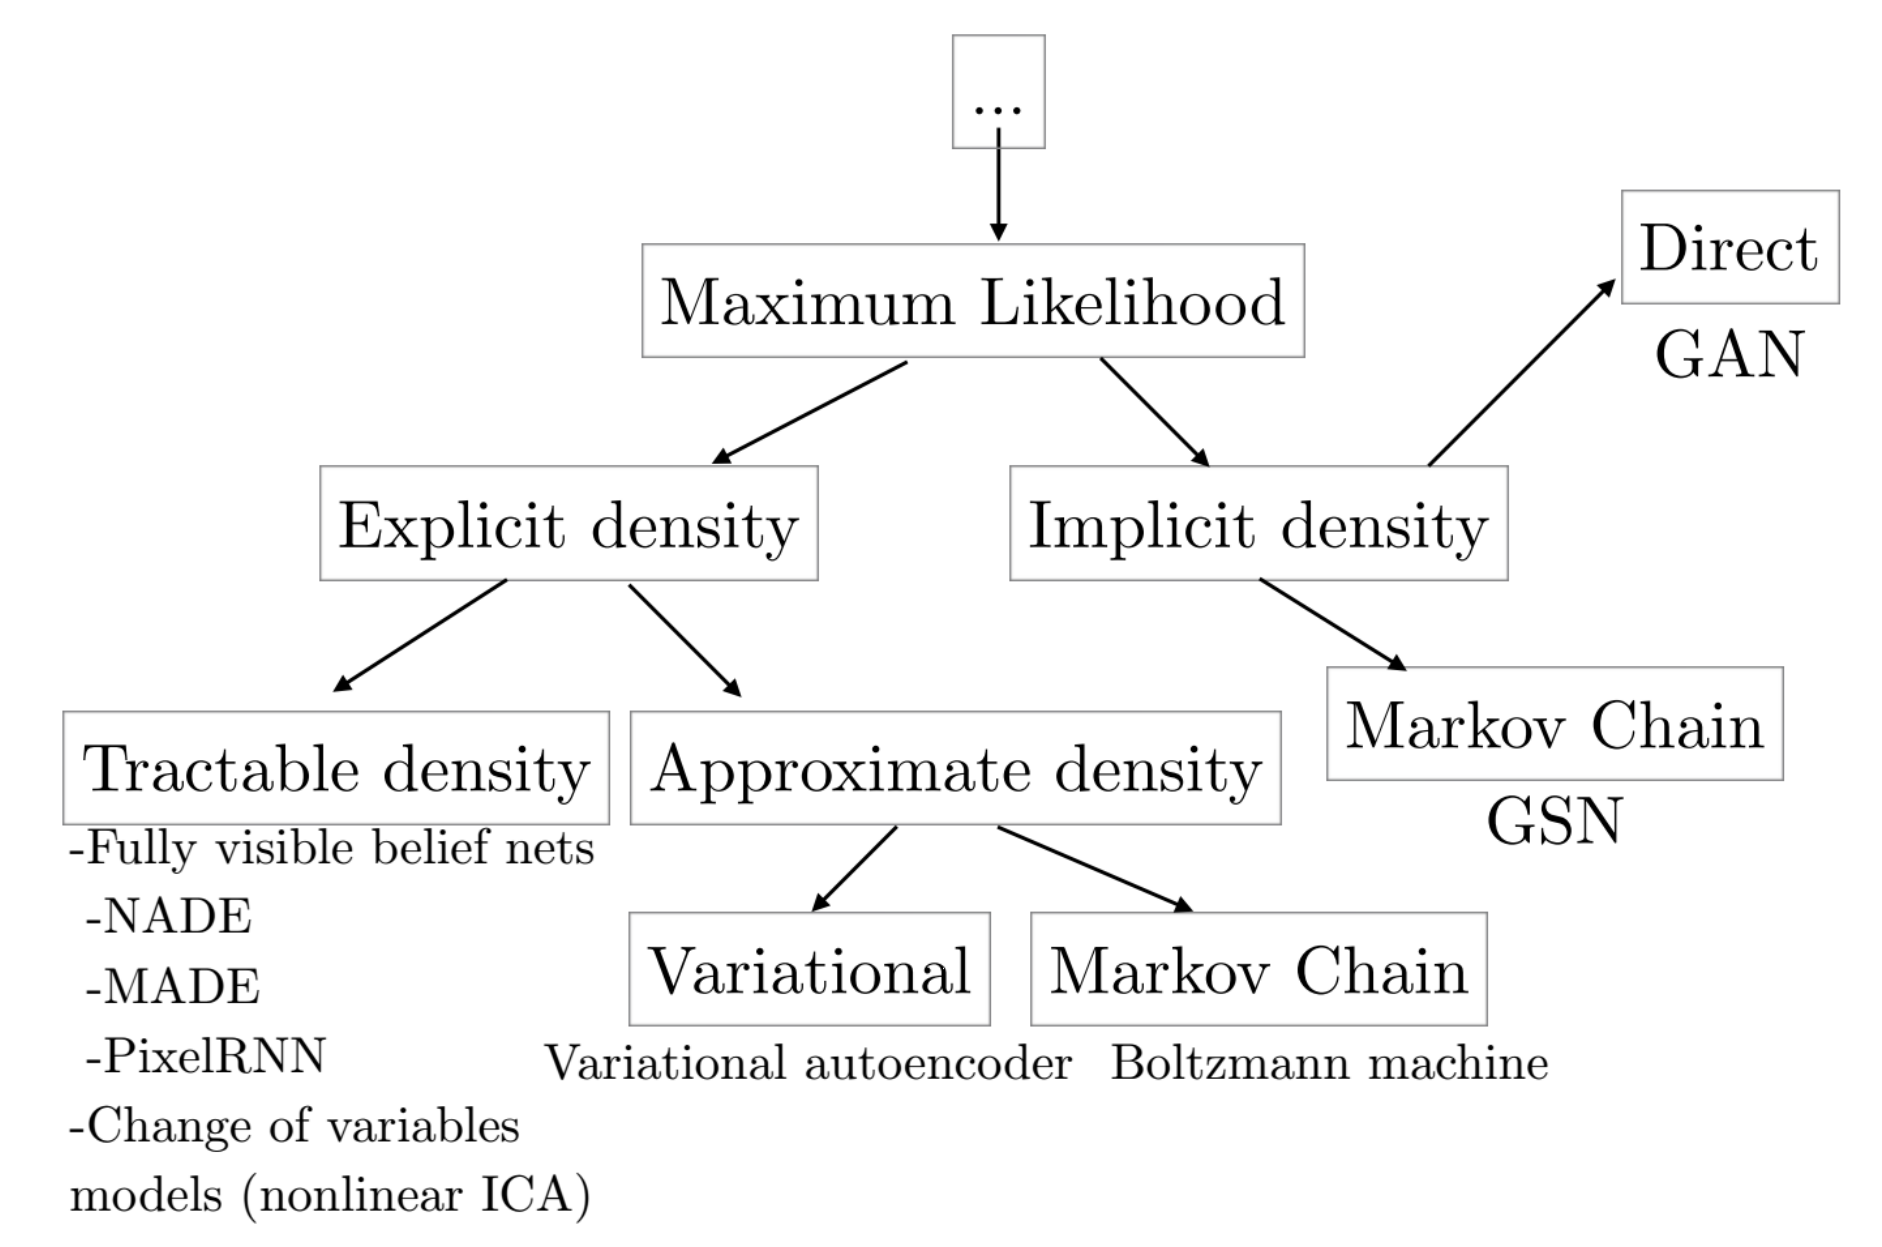
\includegraphics[scale=0.2]{images/gen_models.png}
	\end{center}
		\underline{GAN}: implicit model, adversarial training. Mini-max game:\\ $\min_G \max_D V(G,D) = \mathbb{E}_{\bm{x}\sim p_{r}(\bm{x})} \left[\log \left(D\left(\bm{x}\right)\right)\right] + \mathbb{E}_{\bm{z}\sim p_{z}(\bm{z})} \left[\log\left(1 - D\left(G\left(\bm{z}\right)\right)\right)\right] $. Better loss for generator: $-\log D(G(z))$. Otherwise vanishing gradients if D too strong.\\[2pt]
	\textit{Problems}: reaching equilibrium (oscillation around Nash), mode collapse if $\partial \loss / \partial z\approx 0$, low dimensional support (JS assumes overlap of distributions).\\[2pt]
	\textit{Improvements}: WGAN using Earth-Mover's distance (also good for non-overlapping), usage of labels $y$ like in conditional GANs, label smoothing for overconfident D, Virtual BatchNorm with reference batch to reduce intra-batch inference\\[4pt]
	\underline{Boltzmann machines}: Pdf based on energy function we learn: $p(x)=1/Z \exp(-E(x))$ where $Z=\sum_{x'} \exp(E(x'))$. $Z$ complex, $2^{n}$ pos. for binary data. Restrain to pairwise relations: $E(x)=-x^TWx-b^Tx$. \textit{Restricted BM}: reduce $W$ by introducing $h$ latents: $E(x,h)=-x^TWh-b^Tx-c^Th$, $p(x)=1/Z\sum_{h'} \exp(-E(x,h'))$, higher-order relations. Can reformulate to $p(h_j|x,\theta)=\sigma(W_{:,j}x+b_j)$, $p(x_i|h,\theta)=\sigma(W_{i,:}h+c_i)$. Maximize log likelihood by contrastive divergence. Sample $h_0\sim p(h|x)$, $x_1\sim p(x|h_0)$, a.s.o.\\[4pt]
	\underline{VAE}: Model $p(x,z)=p(x|z)p(z)$. Goal is to maximize $p(x)=\int p(x,z)dz$ which is intractable. Use ELBO instead:\\
	$\log p(x) > \mathbb{E}_{q_{\varphi}(z|x)}\left[\log p_{\theta}(x|z)\right] - \text{KL}\left(q_{\varphi}(z|x)||p_{\lambda}(z)\right)$\\
	Difference is $ - \text{KL}\left(q_{\varphi}(z|x)||p(z|x)\right)$. \\
	
	\textit{Reparameterization trick}: sample from external dist., and transform it to own. For Gaussian: $z=\mu_q + \epsilon \cdot \sigma_q$. Backprop through model params and lower variance than REINFORCE.\\
	\end{minipage}
};
%------------ COMANDOS DE TEXTO BOX ---------------------
\node[fancytitle, right=10pt] at (box.north west) {Deep Generative Models (1)};
\end{tikzpicture}
%------------ CONTEÚDO COMANDOS DE TEXTO ---------------------
\begin{tikzpicture}
\node [mybox] (box){%
	\begin{minipage}{0.3\textwidth}
	\textit{Improvements}: $q(z|x)$ with NF on top, ELBO is extended by NF term. Optimize prior $p_{\lambda}(z)=\frac{1}{K}\sum_k q_{\varphi}\left(z|u_k\right)$, $u_k$ trained\\[4pt]
	\underline{NF}: Model $p(x)$ directly with series of invertible transformations shifting probability mass. Math expression of NF:\\
	 $x = z_k = f_k \circ f_{k-1} \circ ... \circ f_1 (z_0) \to z_i = f_i(z_{i-1})$\\
	 $p(z_i) = p(z_{i-1}) \cdot \left|\det \frac{f_{i}^{-1}}{z_i}\right| \implies p(x) = p(z_0) \cdot \prod_{i=1}^{K} \left|\det \frac{f_{i}^{-1}}{z_i}\right|$\\
	 $\log p(x) = \log p(z_0) - \sum_{i=1}^{K} \log \left|\det \frac{f_{i}}{z_i}\right|$\\
	 $f$ must be invertible and has simple $\det$ Jacobian (triangular)
	\end{minipage}
};
%------------ COMANDOS DE TEXTO BOX ---------------------
\node[fancytitle, right=10pt] at (box.north west) {Deep Generative Models (2)};
\end{tikzpicture}

\begin{tikzpicture}
\node [mybox] (box){%
	\begin{minipage}{0.3\textwidth}
	Hold dist. per latent variable instead of single val. \textit{Benefits}: ensemble modeling (better acc), uncertainty estimates, prevent overconfidence, model compression (prior towards 0)\\[4pt]
	\underline{Epistemic uncertainty}: dataset limits, unseen data, important for safety-critical and small datasets. Posterior $p(w|x,y)$ intractable. \textit{MC dropout}: apply DP during test (Bernoulli-dist over weights). Var approx. uncertainty. Any NN can be made Bayesian with that, but expensive and not accurate. Can also be motivated from Gaussian Processes. Over-param. models better uncert. estm.\\[4pt]
	\underline{Aleatoric uncertainty}: data uncertainty due to noise (e.g. bad sensor). \textit{Data-dependent/heteroscedastic}: specific raw inputs hard to interpret, predict uncert. per data point: $\loss = \frac{||y_i - \hat{y}_i||^2}{2\sigma_i^2} + \log \sigma_i$. \textit{Task-dependent/homoscedastic}: introduced by task (e.g. depth estimation), Sol: train on multiple tasks. $\loss = \frac{||y_i - \hat{y}_i||^2}{2\sigma^2} + \log \sigma$
	\end{minipage}
};
%------------ COMANDOS DE TEXTO BOX ---------------------
\node[fancytitle, right=10pt] at (box.north west) {Bayesian Deep Learning (1)};
\end{tikzpicture}

\begin{tikzpicture}
\node [mybox] (box){%
	\begin{minipage}{0.3\textwidth}
	\underline{Bayes by Backprop}: approx. true posterior $p(w|\mathcal{D})$ by $q(w|\theta)$: $\loss = \log q(w_s|\theta) - \log p(w_s) - \log p(\mathcal{D}|w_s) \hspace{2mm}\text{ where }\hspace{2mm} w_s\sim q(w_s|\theta)$\\
	Example: assume Gaussian variational posterior with softplus $w=\mu + \epsilon\cdot \log\left(1+\exp\rho\right)$, then learn $\mu$ and $\rho$ by SGD.
	\end{minipage}
};
%------------ COMANDOS DE TEXTO BOX ---------------------
\node[fancytitle, right=10pt] at (box.north west) {Bayesian Deep Learning (2)};
\end{tikzpicture}

\begin{tikzpicture}
\node [mybox] (box){%
	\begin{minipage}{0.3\textwidth}
	\underline{Autoregressive Models}: generative without latent variables, assuming order in data, conditional probs $p(x) = \prod_k p(x_k|x_{<k})$. Not necessarily parameter sharing, $p(x)$ tractable, but slow\\[4pt]
	\underline{NADE}: model output with single layer, $\mathcal{O}(D\times H)$ params\\$p(x_d=1|x_{<d})=\sigma\left(V_{d,:}\cdot h_d+b_d\right)$, $h_d=\sigma\left(W_{:,<d}\cdot x_{<d} + c\right)$\\
	\underline{MADE}: Autoencoder with carefully masked connections. $y_d$ only depends on $x_{<d}$. Connections can be shared with future $d$\\[4pt]
	\underline{PixelRNN}: row-wise pixel and sequential color generation\\
	$p(x_i|x_{<i}) = p(x_{i,R}|x_{<i})\cdot p(x_{i,G}|x_{i,R}, x_{<i})\cdot p(x_{i,B}|x_{i,R}, x_{i,G}, x_{<i})$\\
	\textit{Row-LSTM}: next output depends on three hidden states above\\
	\textit{Diagonal-BiLSTM}: use all pixels before (all prev rows and left)\\
	\underline{PixelCNN}: masked convs to only see top and left. Causes blind spot. Use separated vertical and horizontal stack\\[4pt]
	\underline{PixelVAE}: Standard VAE with PixelCNN as decoder
		\begin{minipage}{\textwidth}
	\centering
	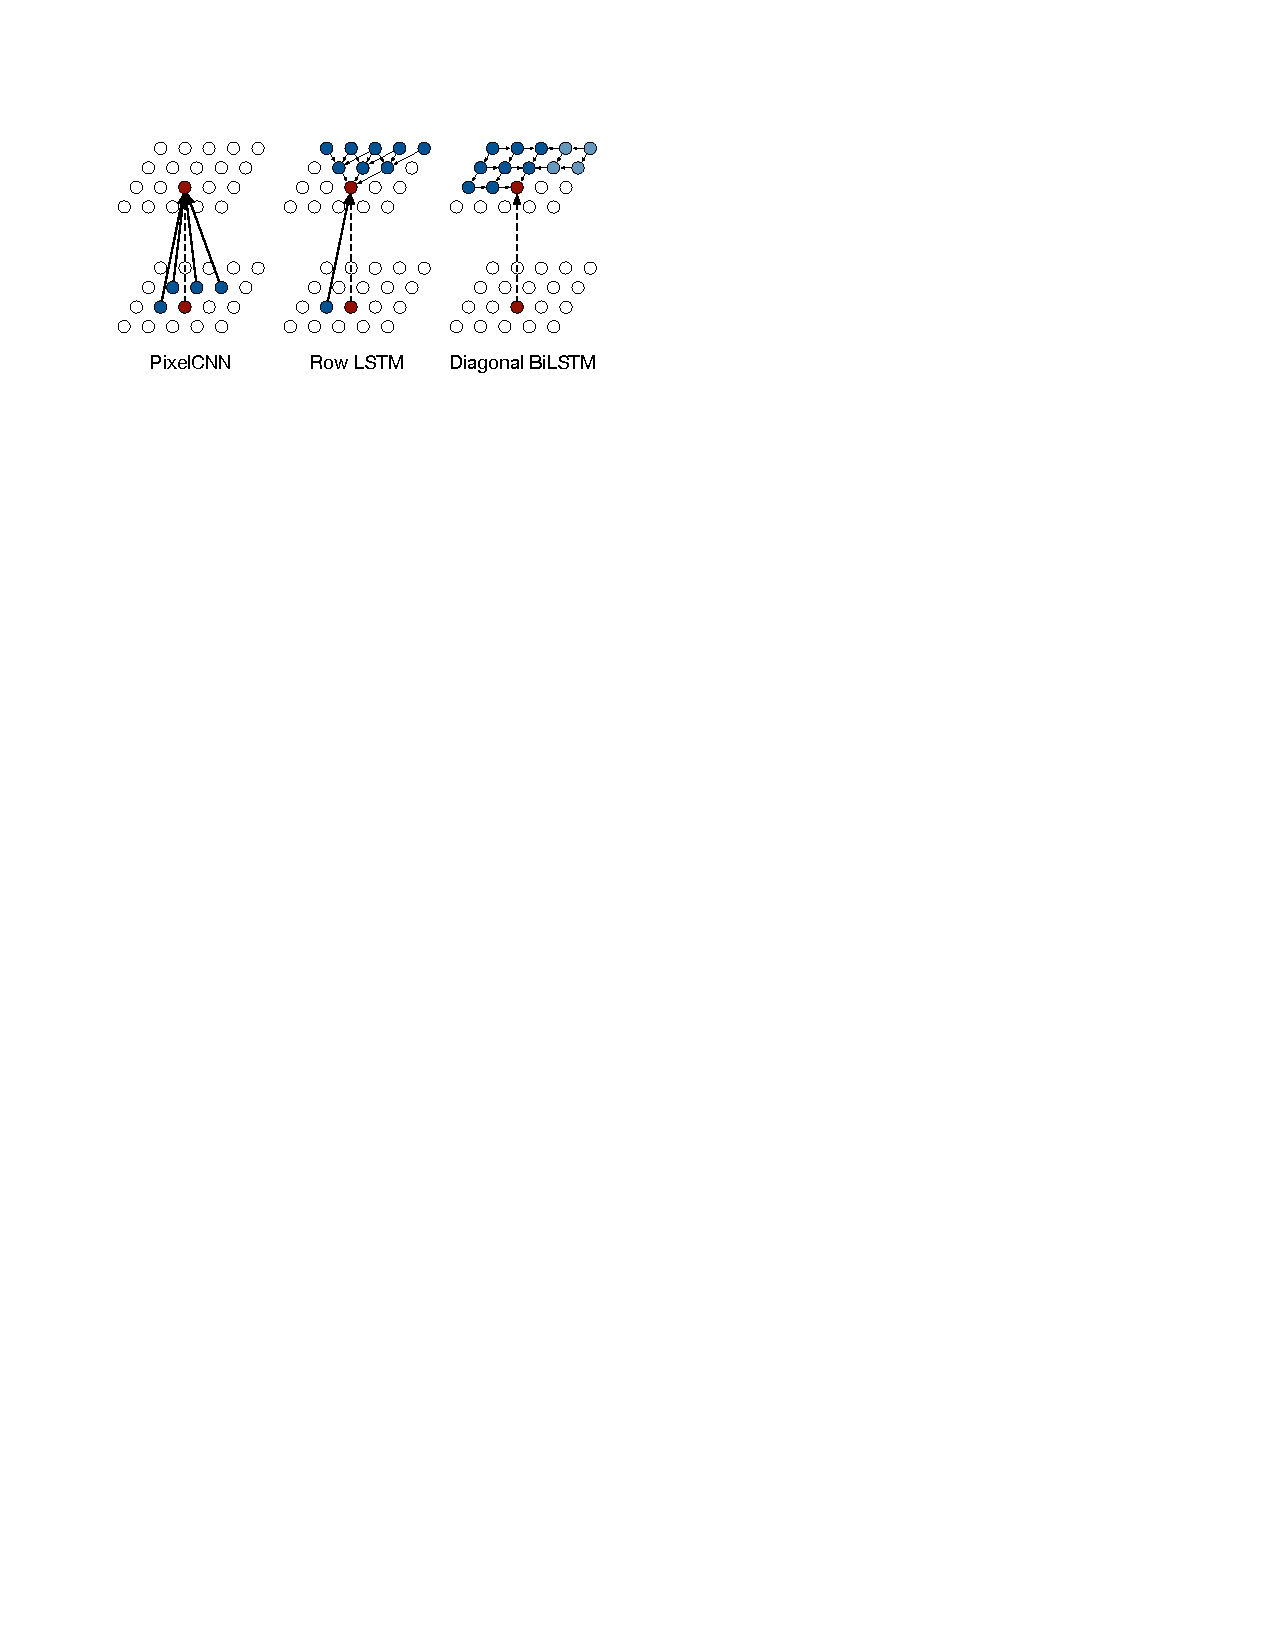
\includegraphics[width=0.3\textwidth]{images/Autoregressive_PixelRNN.pdf}
	\end{minipage}
	
	\end{minipage}
};
%------------ COMANDOS DE TEXTO BOX ---------------------
\node[fancytitle, right=10pt] at (box.north west) {Deep Sequential Models};
\end{tikzpicture}

\begin{tikzpicture}
\node [mybox] (box){%
	\begin{minipage}{0.3\textwidth}
	Value function $q^{\pi}(s_t, a_t) = \mathbb{E}_{\pi}\left[r_{t+1}+\gamma r_{t+2} + \gamma^2 r_{t+3} + ... | s_t, a_t\right]$\\
	Bellman equation $q^{\pi}(s_t, a_t) = \mathbb{E}_{\pi}\left[r_{t+1}+\gamma q^{\pi}| s_t, a_t\right]$\\
	Optimal policy with $q^{*}(s_t,a_t) = r_{t+1} + \gamma \max_{a_{t+1}} q(s_{t+1}, a_{t+1})$\\[4pt]
	\underline{Value-based}: learn $q^{*}$ to get $\pi^{*}$. Q-Learning (off-policy):\\
	$\mathcal{L} = \mathbb{E}\left[\left(r + \gamma \max_{a_{t+1}} q(s_{t+1}, a_{t+1}, \theta) -q(s_{t}, a_{t}, \theta) \right)^2\right]$\\
	For gradient calculation, bootstrapped val is fixed. \\
	\underline{Stability problems}: bootstrap, target and policy always changing, oscillations; seq. data break iid assump.; scale of $q$ values hard to control, unstable gradients; \\
	\underline{Solutions}: experience replay (store samples $\langle s, a, r, s'\rangle$ in dataset, sample from that, makes batch iid), freezing target network every $K$ iters to avoid oscillations, clip rewards, skip frames, control exploration vs. exploitation by annealing $\epsilon$-greedy policy\\[4pt]
	\underline{Policy-based}: learn $\pi^{*}$ directly, avoid problems with $q$ vals (especially hard for continuous action space). Training steps:\\
	\vspace{-3mm}
	\begin{enumerate}[leftmargin=4mm]
	\setlength\itemsep{0.0em}
	\item Determine $q$ by simulation: $q^{\pi_w}(s_t, a_t) = \mathbb{E}\left[r_t + \gamma r_{t+1}... | \pi_{w}\right]$
	\item Maximize $q$ by $\pd{\mathcal{L}}{w} = \mathbb{E}\left[\chain{q^{\pi}(s,a)}{a}{w}\right]$ (deterministic)\\
	or $\pd{\mathcal{L}}{w} = \mathbb{E}\left[\pd{\log \pi^{w}(a|s)}{w} q^{\pi}(s,a)\right]$ (stochastic)
	\end{enumerate}
	\textit{Asynchronous Advantage Actor-Critic}: Learn both policy and value function at same time, run multiple agents simultaneously (more diverse samples), advantage estimates: use learned value function to compare actually gained $q$ value. If loss is higher, unexpected (good) things happened $\Rightarrow$ exploration\\[4pt]
	\underline{Model-based}: try to model environment and be aware of rules. E.g. AlphaGo with tree-search guided by CNNs. Two policy networks playing against each other, and a third network to predict $V(s_t)=\sum_{a'} \pi(a'|s_t) \cdot q^{\pi}(s_t, a')$.
	\end{minipage}
};

	
%------------ COMANDOS DE TEXTO BOX ---------------------
\node[fancytitle, right=10pt] at (box.north west) {Deep Reinforcement Learning};
\end{tikzpicture}

\begin{tikzpicture}
\node [mybox] (box){%
	\begin{minipage}{0.3\textwidth}
	Forward KL, $D_{KL}(p||q)$, \textit{overestimates} the variance of the true posterior $P$ by assigning a high probablity mass to our approximate posterior $q$ everywhere that ``the data occurs'' [everywhere $P$ has some probability mass]. \\
		$D_{KL}(p||q) = \int p(x) \log \frac{p(x)}{q(x)}dx \Rightarrow$ if $p(x)>0$, then $q(x)>0$\\[4pt]
		
	Backward KL, $D_{KL}(q||p)$, \textit{underestimates} the variance of $P$ by assignming low probaility mass to $q$ everywhere ``data does not occur'' [everywhere $P$ has no probability mass].\\
		$D_{KL}(q||p) = \int q(x) \log \frac{q(x)}{p(x)}dx \Rightarrow$ if $p(x)=0$, then $q(x)=0$\\
		
	$ a = Wx+b$, $\pd{a_i}{W_{jk}} = 1(i=j)\cdot x_k$, $\pd{a}{b} = \bm{I}$, and $\pd{a}{x} = W$\\
	\end{minipage}
};
%------------ COMANDOS DE TEXTO BOX ---------------------
\node[fancytitle, right=10pt] at (box.north west) {Math to know};
\end{tikzpicture}

\begin{tikzpicture}
\node [mybox] (box){%
	\begin{minipage}{0.3\textwidth}
	\underline{Compare non-linear activation functions}
	% \vspace{-3mm}
	\begin{description}[leftmargin=4mm]
	\setlength\itemsep{0.0em}
	\item[ReLU] Neural Network is a directed acyclic graph		
	% \item Every module can be expressed by $a=h(x;w)$
	\item[sigmoid] Use loss function that matches output distribution to improve numerical stability and make gradients larger
	\item[tanh] Input and output distribution of every module should be the same to prevent inconsistent behavior and harder learning
	\end{description}
	\end{minipage}
};
%------------ COMANDOS DE TEXTO BOX ---------------------
\node[fancytitle, right=10pt] at (box.north west) {Old Exams};
\end{tikzpicture}

\begin{tikzpicture}
\node [mybox] (box){%
	\begin{minipage}{0.3\textwidth}
	\underline{Differences between generative and discriminative models}\\
	1. Generative models are used to estimate the joint probability density function $p(x)$. Discriminative models are used, instead, to model the conditional $p(y|x)$.\\
	2. Generative models are often intractable because in the $p(x)=\int p(x|z) p(z) dz$ the integral is not always possible to analytically compute.\\
	3. Discriminative models tend to yield better accuracies given a task, meaning they are optimized for the particular task, at the cost of potential overfitting.\\[5pt]
	\underline{Advantages/Disadvantages of generative models}\\
	\textbf{GAN}: Very good, realistic results, fast to sample from, no need to train on likelihood, very flexible to extension \textit{Drawbacks}: no quantitative evaluation, hard to train (sensitive to hyperparameters, mode collapse, etc.), no real objective in terms of likelihood (and distribution is unknown)\\
	\textbf{VAE}: \textit{Benefits}: Usable for data compression, distribution known (calculate likelihood function), stable training (no mode collapse) \textit{Drawbacks}: only approx. likelihood (ELBO), tends to give blurry instead of realistic images, need flexible enough encoder and prior\\
	\textbf{NF}: \textit{Benefits}: directly optimize $p(x)$, one-to-one mapping between $z$ and $x$ (knows exact embedding of any image in latent space) \textit{Drawbacks}: high number of parameters, complexity restrained by requirement of reversible $f$\\[5pt]
	\underline{Difference RNN/Autoregressive}\\
	\textbf{RNN}: shares weigths over steps, applicable to any sequence length, compresses all previous inputs into single hidden state/memory, not necessarily generative\\
	\textbf{Autoregressive}: does not necessarily share weights, fixed in sequence length, are generative
	\end{minipage}
};
%------------ COMANDOS DE TEXTO BOX ---------------------
\node[fancytitle, right=10pt] at (box.north west) {Additional questions};
\end{tikzpicture}

\begin{tikzpicture}
\node [mybox] (box){%
	\begin{minipage}{0.3\textwidth}
	\begin{minipage}{0.45\textwidth}
	\includegraphics[width=\textwidth]{images/NN_Zoo.png}
	\end{minipage}
	\begin{minipage}{0.45\textwidth}
	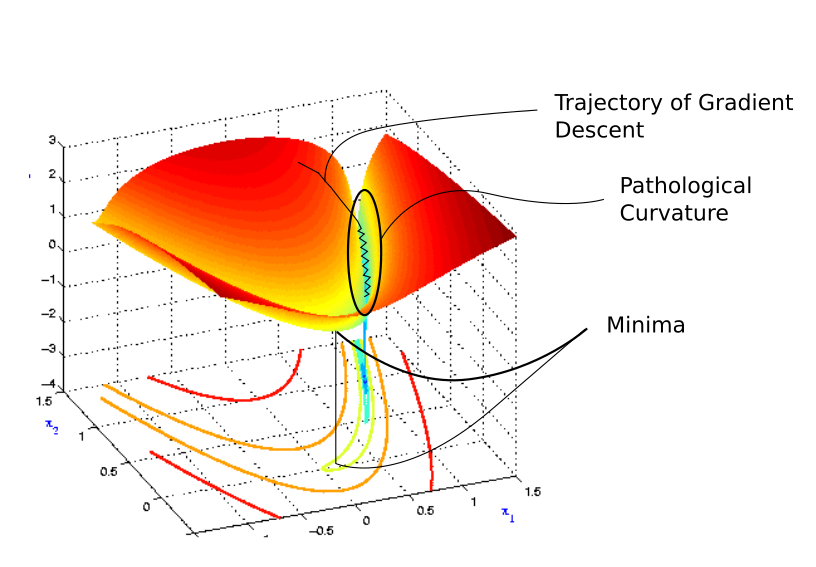
\includegraphics[width=\textwidth]{images/optimization_pathological_curvatures.png}
	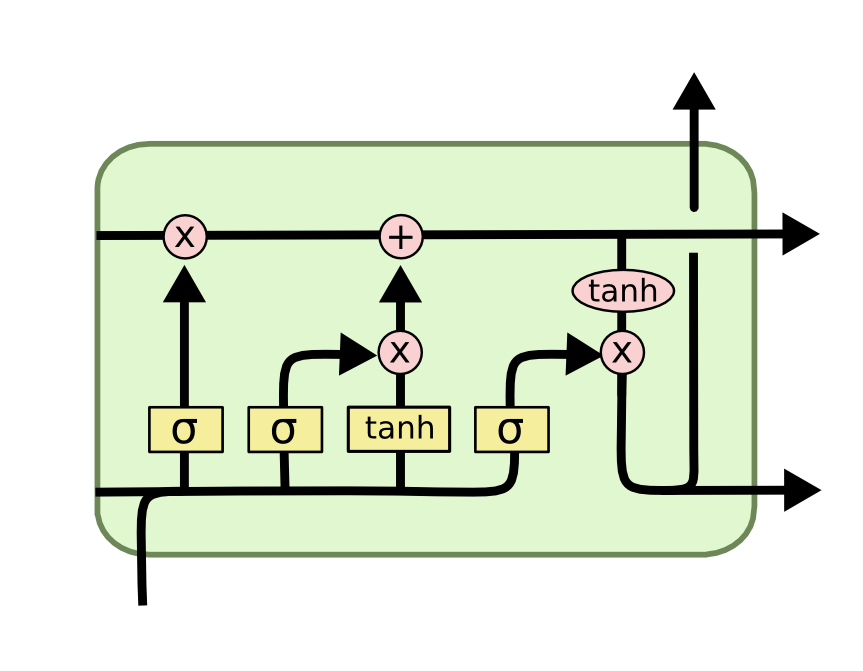
\includegraphics[width=\textwidth]{images/RNN_LSTM.png}
	\end{minipage}
	\\
	\begin{minipage}{0.9\textwidth}
	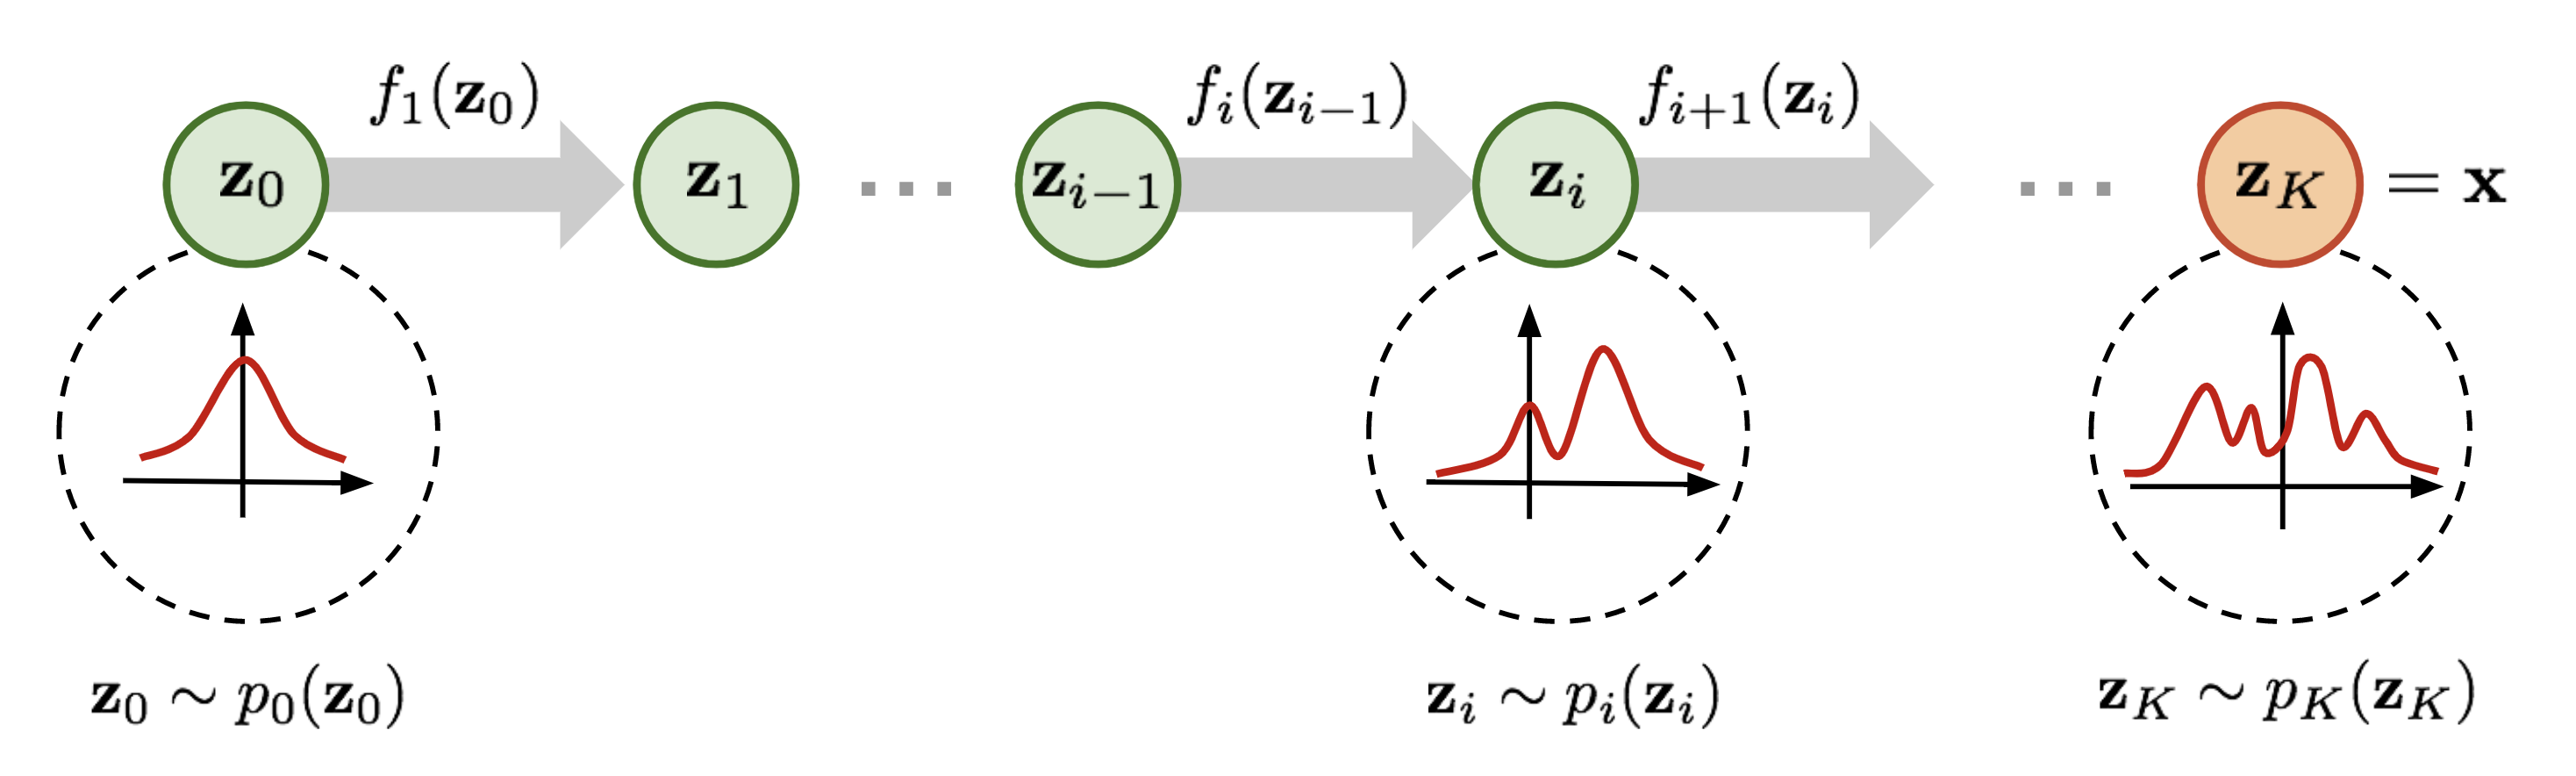
\includegraphics[width=\textwidth]{images/NF_concept.png}
	\end{minipage}
	
%	\begin{minipage}{\textwidth}
%	\centering
%	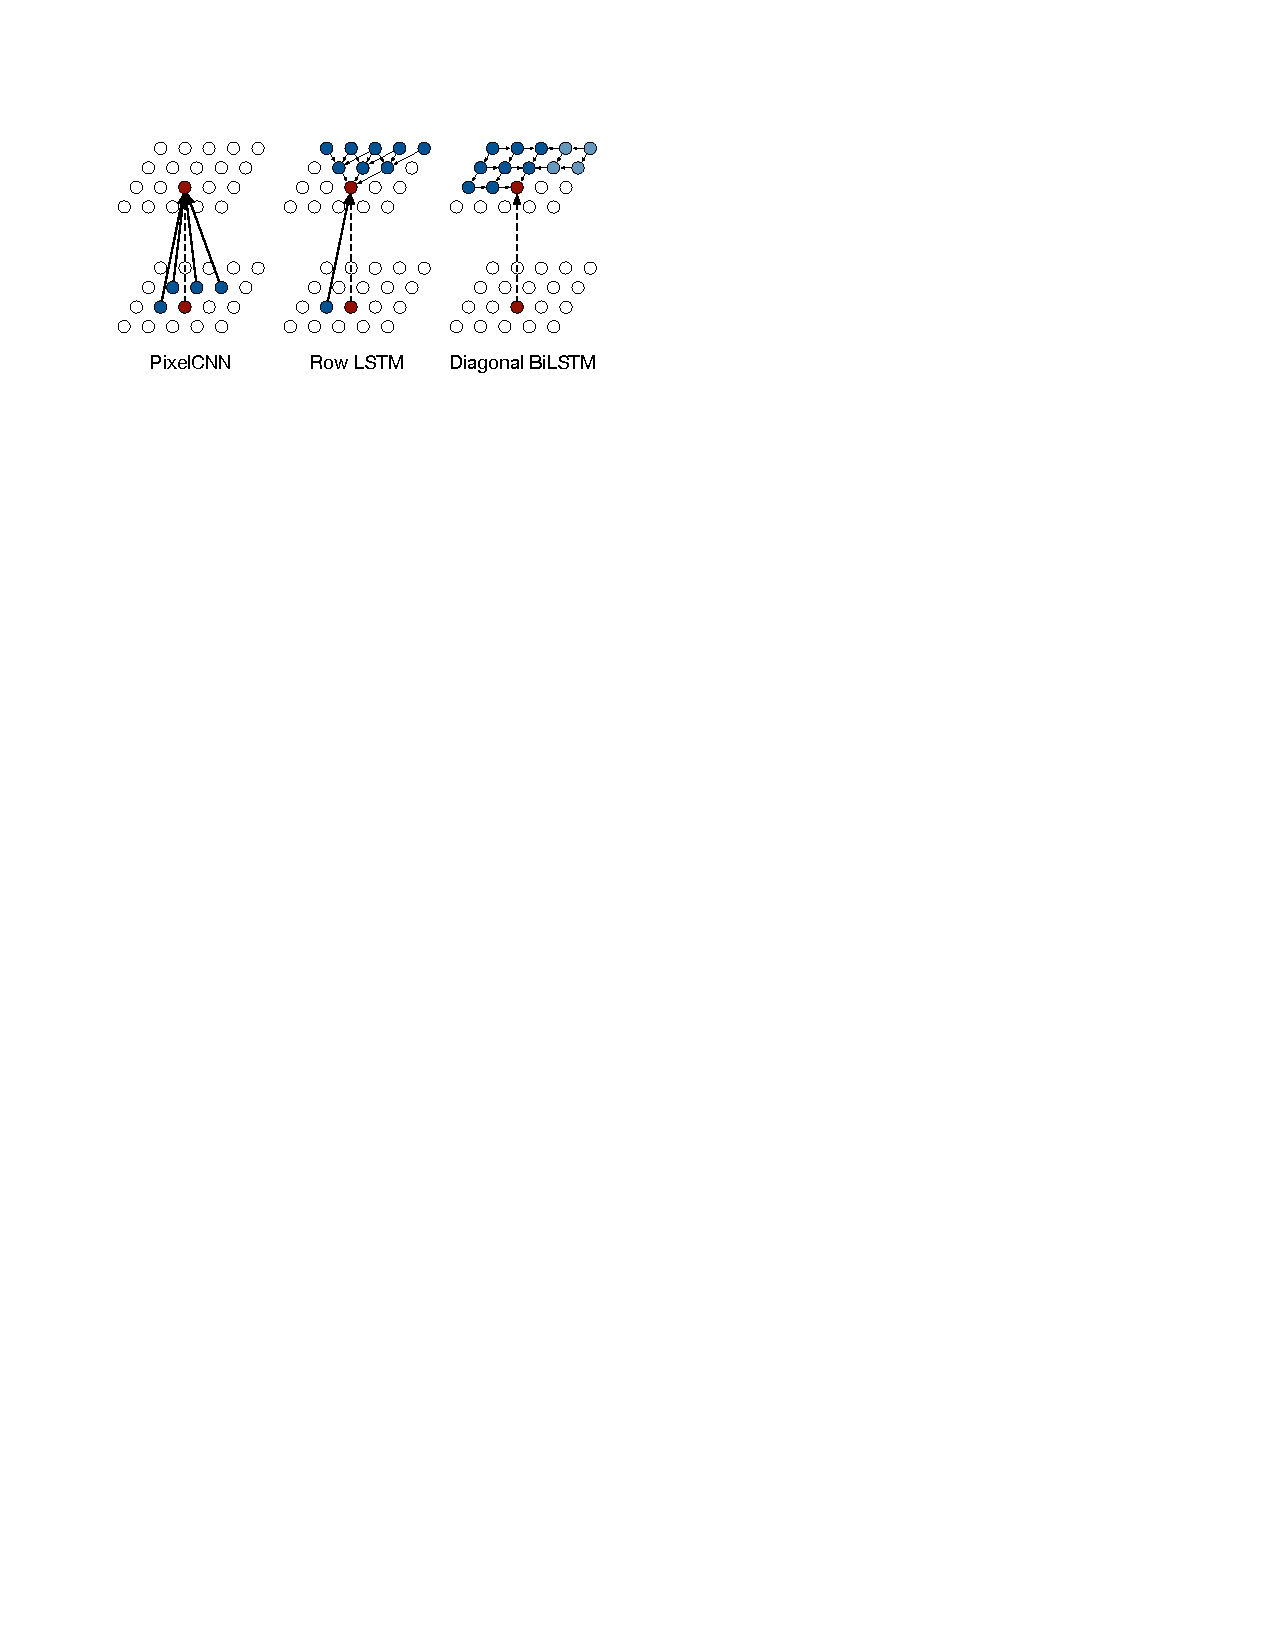
\includegraphics[width=0.7\textwidth]{images/Autoregressive_PixelRNN.pdf}
%	\end{minipage}
	
	\end{minipage}
};
%------------ COMANDOS DE TEXTO BOX ---------------------
\node[fancytitle, right=10pt] at (box.north west) {Figures};
\end{tikzpicture}

%\begin{tikzpicture}
%\node [mybox] (box){%
%	\begin{minipage}{0.3\textwidth}
%	\includegraphics[width=0.5\textwidth]{figures/NN_Zoo.png}
%	\end{minipage}
%};
%%------------ COMANDOS DE TEXTO BOX ---------------------
%\node[fancytitle, right=10pt] at (box.north west) {NN Zoo};
%\end{tikzpicture}

\end{multicols*}
\end{document}